% !TeX spellcheck = fr_FR
\documentclass{beamer}
\usetheme{metropolis}
\usepackage{appendixnumberbeamer}

\metroset{
	sectionpage=none,
	progressbar=frametitle
}

\setbeamercolor{background canvas}{bg=white}

\usepackage{polyglossia}
\setdefaultlanguage{french}
\usepackage{mathtools,amsfonts,amssymb}
\usepackage{booktabs}
\usepackage{enumitem}

\usepackage{csquotes}
\usepackage[
	backend=biber,
	sorting=nyt
]{biblatex}
\addbibresource{../rapport/references.bib}

\usepackage{dsfont}
\usepackage{stmaryrd}
\usepackage{graphicx}
\usepackage{subcaption}
\usepackage{siunitx}

\usepackage{hyperref}
\usepackage{cleveref}

\newcommand{\RR}{\mathbb{R}}
\newcommand{\NN}{\mathbb{N}}
\newcommand{\ZZ}{\mathbb{Z}}
\newcommand{\PP}{\mathbb{P}}
\newcommand{\EE}{\mathbb{E}}
\newcommand{\Var}{\mathrm{Var}}

\DeclareMathOperator*{\argmax}{argmax} % no space, limits underneath in displays

\title{
	\textit{Processus ponctuels et réseaux de neurones récurrents}
}
\author{
	Cheikh Fall\\
	Wilson Jallet
}

\date{11 décembre 2018}

\begin{document}
\maketitle

\begin{frame}{Introduction}
Beaucoup de phénomènes se manifestent par des événements ponctuels.\pause

L'arrivée de certains événements peut favoriser l'arrivée d'autres dans le futur.
\end{frame}

\section{Modèles}

\begin{frame}{Modélisation: Processus ponctuels}
Des événements $(t_i, k_i)$ de différents types $k_i\in\llbracket 1, K\rrbracket$ arrivant  aux $t_i$.\pause

Le modèle de \textbf{processus ponctuel}:
\begin{itemize}
	\item[\textbullet] Décompte d'événements $N = (N_t)$ arrivés entre $0$ et $t$ à des instants $t_i$.
	\item[\textbullet] Associé à une \textit{intensité} $\lambda_t$ telle que
	\[
		\EE[dN_t\mid \mathcal{F}_t] = \lambda_t\,dt
	\]\pause
	$\rightarrow$ L'intensité contrôle le flux d'événements.
\end{itemize}

\end{frame}

\begin{frame}{Le modèle classique: Hawkes (\citeyear{hawkes1971})}
\citeauthor{hawkes1971} \cite{hawkes1971} introduit un modèle de processus ponctuel auto-excité
\begin{equation}
\lambda_t =
\underbrace{\mu_t}_{\substack{\text{intensité}\\\text{exogène}}} + \int_0^t \underbrace{g(t-s)}_{\text{noyau}\geq 0}\cdot\, dN_s
\end{equation}
\end{frame}


\begin{frame}{Modélisation par réseaux de neurones récurrents}
Le postulat de base:
\begin{equation}
\lambda_t = f(t\mid \mathcal{F}_t),\quad t \geq 0
\end{equation}
avec $f(\,\cdot \mid \mathcal{F_{.}})$ un réseau de neurones récurrent.\pause

\noindent\textbf{Problème} \begin{itemize}
	\item Processus ponctuel en temps continu $\rightarrow$ RNN en temps continu ?
	\item Choix de $f$? Comment dépendre des paramètres du réseau?
\end{itemize}

\end{frame}

\begin{frame}{Modèle LSTM \autocite{meiEisnerNeuralHawkes}}
\textbf{Idée:} \citeauthor{meiEisnerNeuralHawkes} proposent de choisir 
\begin{equation}
\lambda_t = f(W_\ell h(t))
\end{equation}
avec $h\in\RR^D, D\in\NN^*$ le \textit{hidden state}. Le temps continu est pris en compte par amortissement.
\begin{equation}\label{eq:meiEisnerHiddenStates}
\begin{aligned}
	h(t) &= o_i \odot \tanh(c(t)) \\
	c(t) &= \bar{c}_i + (c_i - \bar{c}_i)e^{-\delta_i(t - t_{i-1})}
\end{aligned} \quad t\in(t_{i-1}, t_i]
\end{equation}
\end{frame}

\begin{frame}
L'\textit{output} $o_i$, le \textit{cell state} initial $c_i$ en $t_{i-1}$ et sa valeur asymptotique $\overline{c}_i$ suivent les équations d'un réseau LSTM classique.

\textbf{Entrées du LSTM:} Pour mettre à jour les paramètres après l'événement $(t_i,k_i)$:\begin{itemize}
	\item[\textbullet] Embedding $x_i\in\RR^K$ du type d'événement
	\item[\textbullet] \textit{Hidden state} $h(t_{i})$ en $t_{i}^{-}$
	\item[\textbullet] \textit{Cell state} $c(t_{i})$ en $t_i^{-}$ (pour calculer $c_{i+1} = c(t_i^{+})$)
	\item[\textbullet] \textit{Cell state} asymptotique $\bar{c}_i$ (pour calculer $\bar{c}_{i+1}$)
\end{itemize}
\end{frame}


\begin{frame}{Variante simplifiée (RNN)}
Une version plus simple avec moins de paramètres du modèle \eqref{eq:meiEisnerHiddenStates}:
\begin{equation}
	h(t) = h_i e^{-\delta_i (t - t_{i-1})}
	\quad t\in (t_{i-1}, t_i]
\end{equation}
où $h_i = h(t_i^{+})$ est calculé en appliquant un réseau RNN simple à l'entrée $(x_i, h(t_i))$.

\end{frame}

\begin{frame}
Ces modèles ont les bonnes propriétés: $(c,h)$, puis $(\lambda_t)$, sont $(\mathcal{F}_t)$-adaptés.

Le nombre de paramètres augmente rapidement entre le RNN et le LSTM (\autoref{fig:networkParamNums}).

\begin{table}
	\begin{tabular}{l|cc}\toprule
	Modèle & $D$ & Nombre de paramètres \\ \midrule
	LSTM & 32 & 7910 \\
	RNN & 64 & 8774 \\
	LSTM & 64 & 30150 \\
	RNN & 128 & 33926 \\
	LSTM & 128 & 117638 \\ \bottomrule
	\end{tabular}\caption{Nombre de paramètres en fonction de la dimension cachée $D$, $K=2$.}\label{fig:networkParamNums}
\end{table}

\end{frame}

\begin{frame}
En théorie, les deux modèles peuvent reproduire les comportement de modèles plus classiques (e.g. Hawkes).

\begin{figure}
	\includegraphics[width=\linewidth]{../notebooks/example_rnnplot2d_hidden128.pdf}
	\caption{Un comportement généré par un modèle RNN non entraîné (poids aléatoires).}\label{fig:untrained1DRNNIntensity}
\end{figure}
	
\end{frame}

\begin{frame}{Apprentissage}
Maximiser la fonction de log-vraisemblance
\begin{equation}\label{eq:logLikelihood}
\begin{aligned}
\ell &= P\left( \{(t_i,k_i)\}_i \mid \Theta \right) \\
&= \sum_{i=1}^{I}\log \lambda^{k_i}_{t_i} - \int_0^T \bar{\lambda}_t\,dt.
\end{aligned}
\end{equation}
avec $\bar{\lambda}_t = \sum_k \lambda^k_t$ l'intensité totale.

\textbf{Remarque} Difficile à calculer!
\end{frame}

\begin{frame}{Prédiction}
On donne un début de séquence $(t_1,k_1)\ldots (t_{i-1}, k_{i-1})$ au réseau pour générer les paramètres pour $(t_{i-1}, t_i]$.
\begin{itemize}
	\item[$\rightarrow$] On peut calculer $\lambda_t = f(t\mid\mathcal{F}_{t_{i-1}})$ pour $t\geq t_{i-1}$
	\item[$\rightarrow$] Permet d'estimer le prochain événement $(t_i, k_i)$
	\[
	\begin{aligned}
		\hat{t}_i &= \EE\left[t_i \middle| \mathcal{F}_{t_{i-1}}\right] \\
		\hat{k}_i &= \argmax_{k}\EE\left[\lambda^k_t/\bar{\lambda}_t\middle| \mathcal{F}_{t_{i-1}} \right]
	\end{aligned}
	\]
\end{itemize}
\end{frame}

\section{Expériences}

\begin{frame}{Expériences}
Dans le rapport $\rightarrow$ difficultés à apprendre des processus au moins multivariés $K\geq 2$.\pause

$\rightarrow$ Erratum dans le calcul de la vraisemblance (corrigé)

\textbf{Expérience 1} Processus de Hawkes bivarié symétrique (noyau exponentiel) sur $[0, 3600]$
\begin{itemize}
	\item $\alpha = \begin{bmatrix}0.1 & 0.01 \\ 0.01 & 0.1\end{bmatrix}$
	\item $\beta = 1$
	\item $\mu_1 = \mu_2 = \num{0.1}$
\end{itemize}
\end{frame}

\begin{frame}
\begin{figure}
	\includegraphics[width=\linewidth]{../results/intensity_baseHawkes2D.pdf}
	\caption{Intensité du processus de Hawkes, généré avec \texttt{tick}.}
\end{figure}
\end{frame}

\begin{frame}
\begin{figure}
	\begin{subfigure}{\linewidth}
		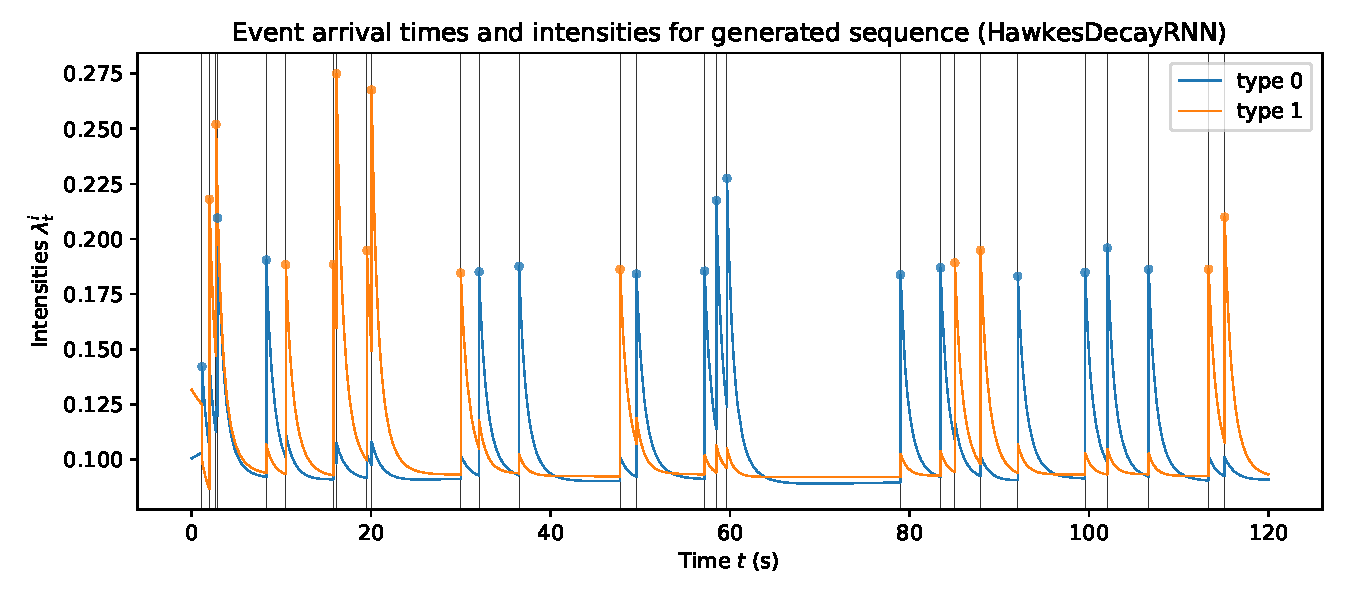
\includegraphics[width=\linewidth]{../results/intensity_HawkesDecayRNN_2d_hidden128_20181209-132014.pdf}
		\caption{Intensité et événements générés par un RNN calibré sur le Hawkes bivarié.}
	\end{subfigure}
	\caption{Intensité apprise par le réseau RNN.}
\end{figure}
\end{frame}

\begin{frame}
\begin{figure}\ContinuedFloat
\begin{subfigure}{\linewidth}
	\includegraphics[width=\linewidth]{../results/intensity_HawkesDecayRNN_2d_hidden64_20181209-003122_OLD.pdf}
	\caption{Avec une erreur d'indice dans le calcul. Le réseau apprend à <<~écraser~>> les autres composantes de l'intensité après chaque événement.}
\end{subfigure}
\end{figure}
\end{frame}

\begin{frame}
\begin{figure}
	\centering
	\includegraphics[width=\linewidth]{../results/2D_Hawkes_Data_RMSE_20181209-181315.pdf}
	\caption{Résultats pour la prédiction d'événements, apprentissage sur des trajectoires d'un Hawkes bivarié ($K=2$).}
\end{figure}
\end{frame}

\begin{frame}
\begin{figure}
	\begin{subfigure}{0.8\linewidth}
		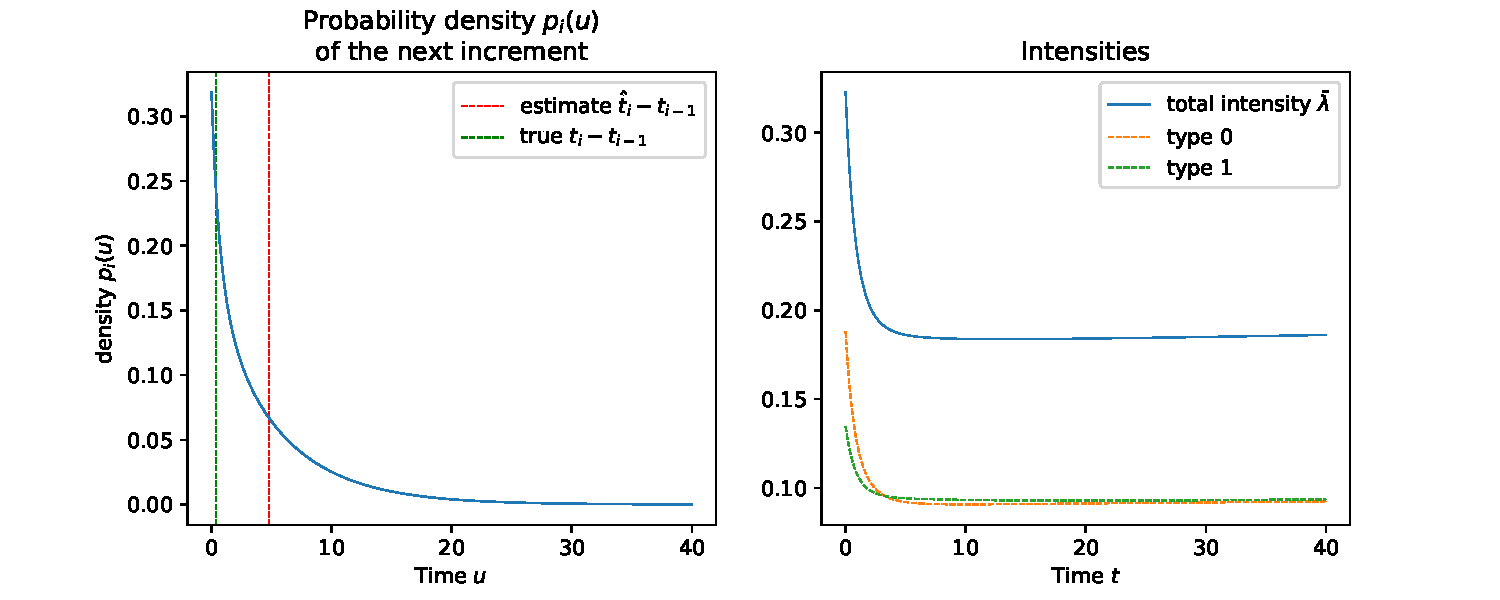
\includegraphics[width=\linewidth]{../notebooks/decayrnn_2d_prediction_graphs_hidden128_NEW.pdf}
		\caption{Le processus de Hawkes sous-jacent est symétrique: pour le prochain événement, les types sont équiprobables.}
	\end{subfigure}
	\begin{subfigure}{0.8\linewidth}
		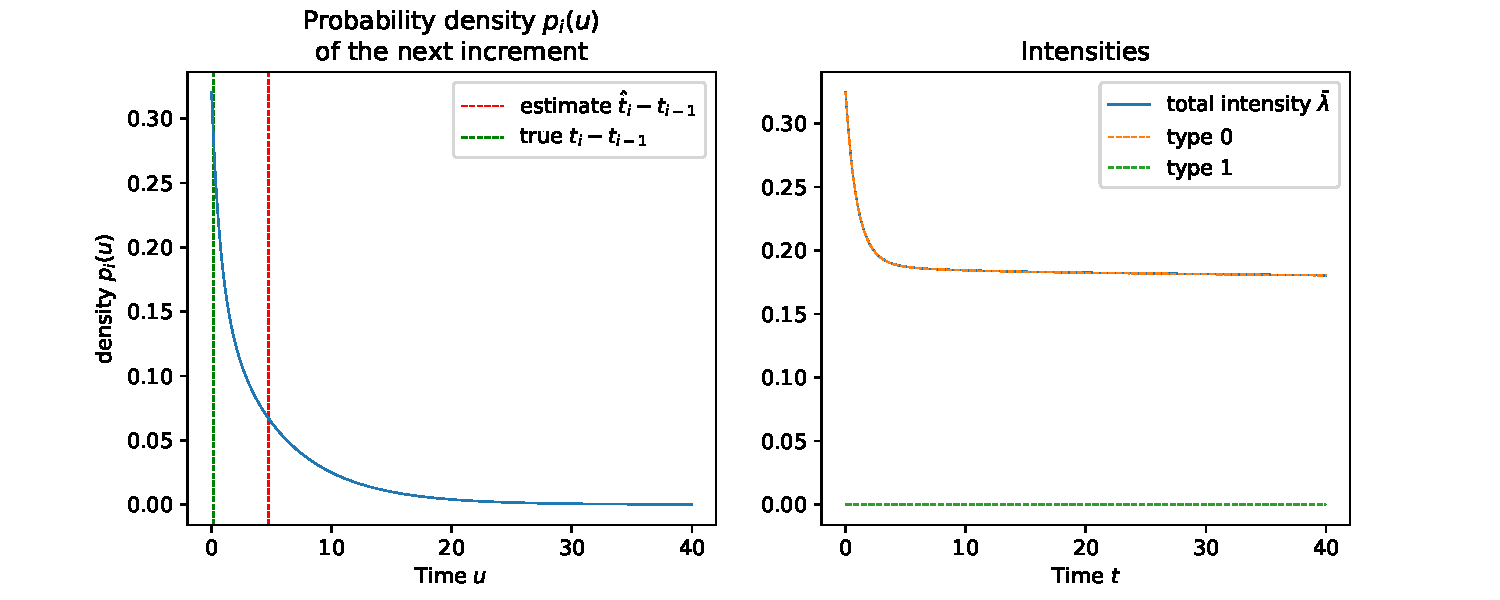
\includegraphics[width=\linewidth]{../notebooks/decayrnn_2d_prediction_graphs.pdf}
		\caption{Avec la faute de calcul. Le type du prochain événement est certainement celui du dernier.}
	\end{subfigure}
\end{figure}
\end{frame}

\begin{frame}
\textbf{Expérience 2} Processus de Hawkes asymétrique, $T = 1800$
\begin{itemize}
	\item $\alpha = \begin{bmatrix}0.1 & 0.07\\ 0.01 & 0.15\end{bmatrix}$
	\item $\beta = 1$
	\item $\mu_1 = \num{0.3} = 3\mu_2$
\end{itemize}
\end{frame}

\begin{frame}
\begin{figure}
	\includegraphics[width=\linewidth]{../results/intensity_baseHawkes2D_asymmetrical.pdf}
	\caption{Intensité du processus généré avec \texttt{tick}.}
\end{figure}
\end{frame}


\section{Conclusion}

\begin{frame}[t,allowframebreaks]{References}
	\printbibliography
\end{frame}

\end{document}
